\documentclass{beamer}
\usetheme{CambridgeUS}

%\usepackage{listings}
%\lstset{language=bash}

\usepackage[english,francais]{babel}
\usepackage[utf8]{inputenc}
%\usepackage[latin1]{inputenc}
\usepackage{verbatim}
%\usepackage{isolatin1}

\title{OAR}
\subtitle{A highly configurable and scalable distributed resources management system}
\author{Olivier~Richard \and Bruno~Bzeznik \and Romain~Cavagna \and Joseph~Emeras}
\institute{ LIG / CIMENT / ALADDIN-G5K }
\date{PORTO ALEGRE - 23/02/2010}


\begin{document}

\frame{
	\titlepage

    \begin{center}

        \includegraphics[height=7ex]{img/oar_logo.png} \\

        
\includegraphics[height=6ex]{img/LIG_coul.jpg}
        \hspace{2ex}
        
\includegraphics[height=3ex]{img/cnrs.jpg}
        \hspace{1ex}
        
\includegraphics[height=3ex]{img/logo_inpg.jpg}
        \hspace{1ex}
        
\includegraphics[height=3ex]{img/inria.jpg} \\
        \hspace{1ex}
        
\includegraphics[height=3ex]{img/logo_ujf.jpg}
        \hspace{1ex}
        
\includegraphics[height=5ex]{img/logo_upmf.jpg}
        \hspace{1ex}
        
\includegraphics[height=2ex]{img/ciment-logo2.jpg}
        \hspace{1ex}
        
\includegraphics[height=5ex]{img/Logo_Aladdin.png}
    \end{center}
	}

\frame{
  \frametitle{Sommaire}
  	\tableofcontents
}

\section{About batch schedulers}

\frame{
 \frametitle{distributed resources management systems}
	
    \begin{itemize}
	\item Also known as {\em Batch Schedulers}
        \item Context: {\bf High Performance Computing}
	\item A lot of them: {\bf Condor }, {\bf Sun Grid Engine (SGE)}, {\bf MAUI/Torque}, {\bf Slurm}, {\bf OAR}, {\bf Catalina}, {\em LSF }, {\bf Lava}, {\em PBS Pro}, {\em Moab}, Loadleveler, CCS...
        \item \url{http://en.wikipedia.org/wiki/Job_scheduler}
  \end{itemize}

}

\begin{frame}
	\frametitle{General concept}

	Generally, they are in 2 layers, sometimes 3 (Workload Managment) :
	
	\begin{center}
			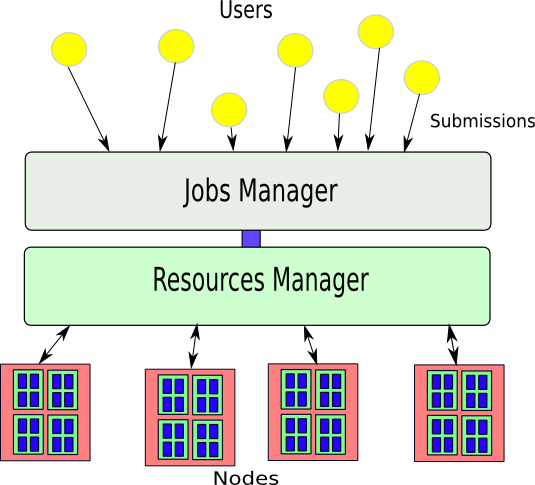
\includegraphics[width=6cm]{img/task_resources.png}
	\end{center}

\end{frame}

\begin{frame}
	\frametitle{General organization}

	\begin{itemize}
		\item A central host
		\item Client programs (command line) to interract with users
		\item A lot of configuration parameters
	\end{itemize}

	\begin{center}
		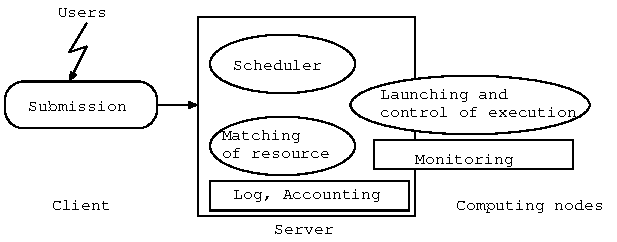
\includegraphics[height=4cm]{Batch_organization.pdf}
	\end{center}

\end{frame}

\section{Common features}

\begin{frame}
\frametitle{Features (1/2)}
	{\bf non-exhaustive list}
		\begin{itemize}
		\item Interactive tasks ({\em submission})(shell) / Batch
		\item Sequential tasks
		\item Walltime limit. ({\bf very important for scheduling!)}
		\item Exclusive / non-exclusive access to resources 
		\item Resources matching
		\item Scripts Epilogue/Prologue (before and after tasks)
		\item {\em Monitoring} of the tasks (resources consumption)
		\item Job dependencies ({\em workflow})
		\item Logging and accounting
		\item Suspend/resume 
	\end{itemize}
\end{frame}

\begin{frame}
\frametitle{Features (2/2)}
	{\bf non-exhaustive list}
		\begin{itemize}
    \item Array jobs
		\item First-Fit (Conservative Backfilling,)
		\item Fairsharing
    \item ... 
		
	\end{itemize}
\end{frame}


\section{OAR objectives and features}


\begin{frame}
	\frametitle{Objectives} \hypertarget{objectifs}{}

	OAR: A {\bf versatile} and {\bf {\em customizable}} batch scheduler.

	\begin{itemize}
		\item Following technological evolutions (machines and infrastructures more and more complicated)
		\item Initial context: CIMENT \hyperlink{ciment-appendix}{ \beamergotobutton{...}}  and Grid5000 \hyperlink{g5k-appendix}{ \beamergotobutton{...}}
                \item Different contexts adaptation (cluster, cluster-on-demand, virtual cluster, multi-cluster, lightweight grid, experimental platform as Grid'5000, {\em big cluster}, special needs). 
	\end{itemize}

\begin{center}
        \hspace{1ex}
        
\includegraphics[height=2ex]{img/ciment-logo2.jpg}
        \hspace{1ex}
        
\includegraphics[height=7ex]{img/Logo_Aladdin.png}
\end{center}

\begin{alertblock}{Under estimation}
   80/20 rule: 20\% features {\bf are not the same for everyone !!!}  
\end{alertblock}

\end{frame}

\frame{
\frametitle{CIMENT local HPC center} \hypertarget{ciment-appendix}{}
  \begin{itemize}
    \item Université Joseph Fourier (Grenoble)
    \item A dozen of heterogeneous supercomputers, more than 2000 cores today
    \item special feature: a lightweight grid (CiGri) making profit of unused cpu cycles through best-effort jobs (a OAR feature)
    \item Great collaborative work production/research
  \end{itemize}
}

\frame{
\frametitle{Grid 5000} \hypertarget{g5k-appendix}{}
  \begin{itemize}
    \item Grid for computing experiments
    \item 9 sites in France + 2 sites abroad
    \item Interconnection gigabit Renater
    \item More than 5000 cores today
  \end{itemize}
}

\frame{
\frametitle{Eco-system}
  \begin{center}
    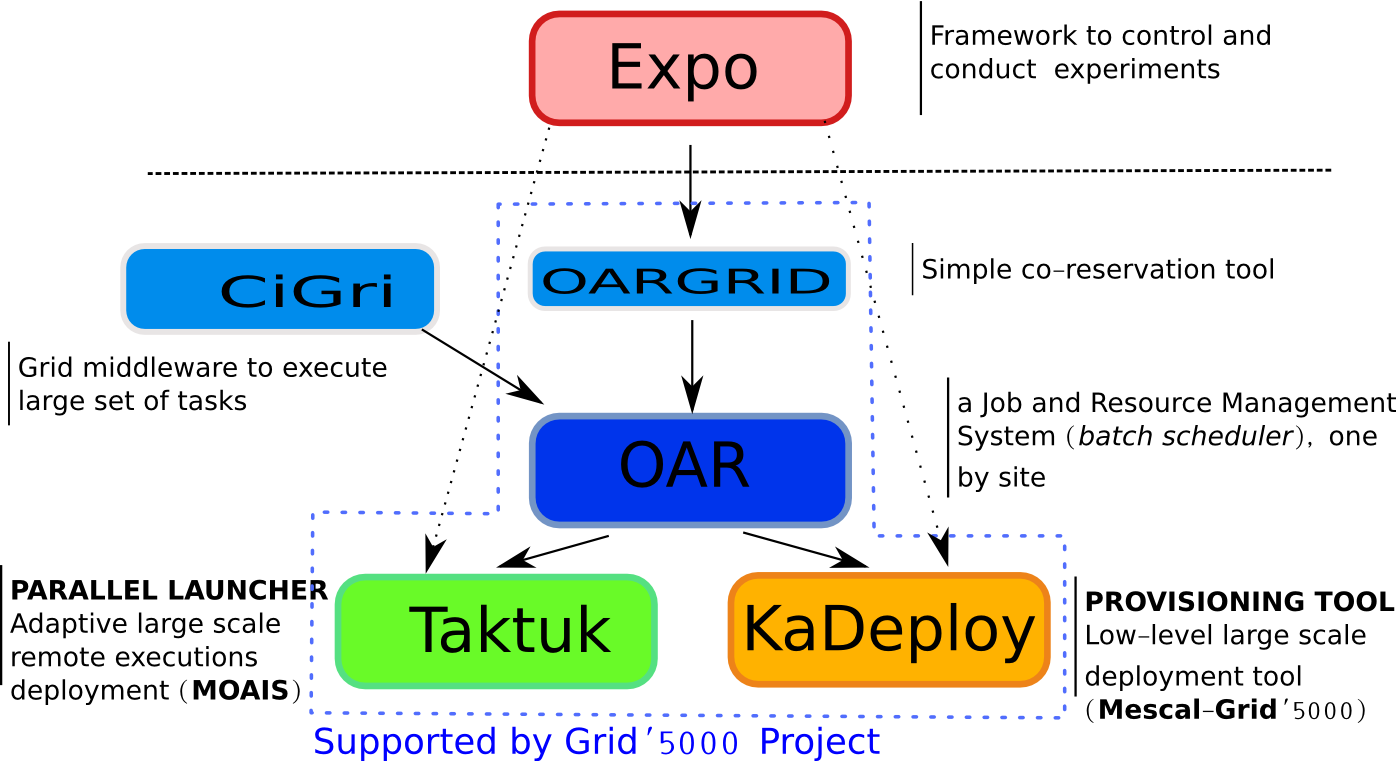
\includegraphics[width=11cm]{global_picture.png}
  \end{center}
}

\begin{frame}
\frametitle{OAR special features}
	{\bf non-exhaustive list}
		\begin{itemize}
    \item Classical features +
    \item Advance Reservation
		\item {\bf Hierarchical expressions into requests }
		\item {\bf Different types of resources (ex licence, storage capacity, network capacity...)  }
		\item {\bf Container tasks} ({\em recursive, task submission inside another task})
		\item {\bf Besteffort tasks} (zero priority task, highly used by {\em CiGri}) 
		\item {\bf Multiple task types} (besteffort, deploy, timesharing, idempotent, power, cosystem ...) (customizable)
    		\item {\bf Moldable tasks}
    		\item {\bf Energy saving}
		%\item First-Fit (Conservative Backfilling,)
		%\item Fairsharing 
		
	\end{itemize}
\end{frame}




\section{Concepts and architecture}
%% Principe
\frame{
  \frametitle{OAR: design concepts}
High level components use
   \begin{itemize}
    \item {\bf Relational database} (MySql/PostgreSQL) as the kernel to store and exchange data
      \begin{itemize}
       \item resources and tasks data
       \item internal state of the system
      \end{itemize}
    \item {\bf Script languages} (Perl, Ruby) for the execution engine and modules
    \begin{itemize}
     \item Well suited for system parts of the code
     \item High level strcutures (lists, hash tables, sort...)
     \item Short developpement cycles
     \end{itemize}
    \item {\bf Other components}: SSH, CPUSETS, Taktuk
    \begin{itemize}
      \item \textbf{SSH, CPUSET} (isolation, cleaning)
      \item \textbf{Taktuk} adaptative parallel launcher 
    \end{itemize}
  \end{itemize}
	\begin{center}
		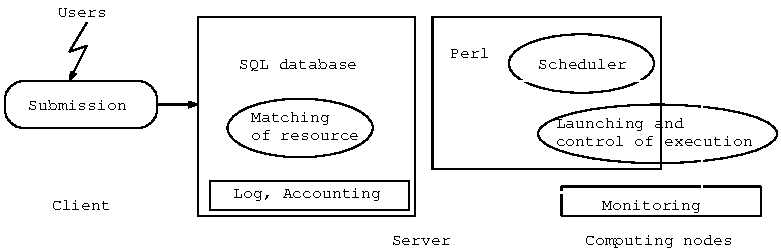
\includegraphics[height=3cm]{OAR_organization.pdf}
	\end{center}

}

\frame{
	\frametitle{OAR : general organisation}
	The database plays a central role

	\begin{itemize}
		\item {\bf internal state easily accessible}
		\item the engine is composed of {\bf little Perl modules}
		\item each module (= a script) easily replaced, maybe in antoher language
	\end{itemize}

	\begin{center}
		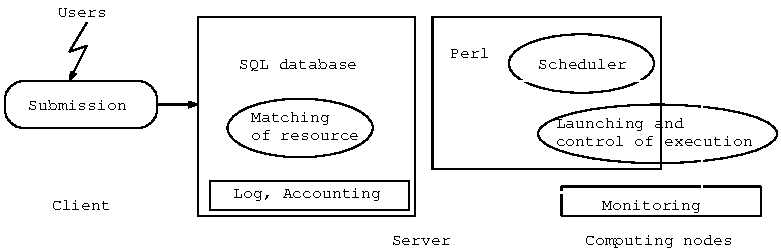
\includegraphics[height=3cm]{OAR_organization.pdf}
	\end{center}
}

\begin{frame}
\frametitle{Job life cycle}
	\begin{center}
		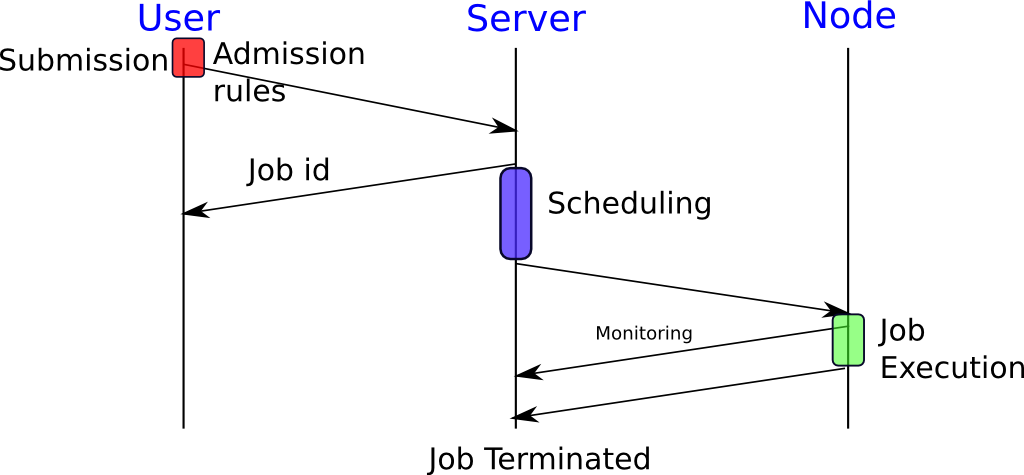
\includegraphics[width=10cm]{cycle_job.png}
	\end{center}
\end{frame}


\frame{
  \frametitle{Admission rules}
  \begin{alertblock}{Very important customization point}
    \begin{itemize}
      \item High {\em customizaton} offered to the administrator
      \item {\bf }manage the requests' scope
      \item default values fixing: walltime, queue, number of resources,..
      \item access control (users, groups, timetable...)
    \end{itemize}
  \end{alertblock}
}


\frame{
	\frametitle{Task status diagram}
	%Exemple du système OAR (version 1.6)
	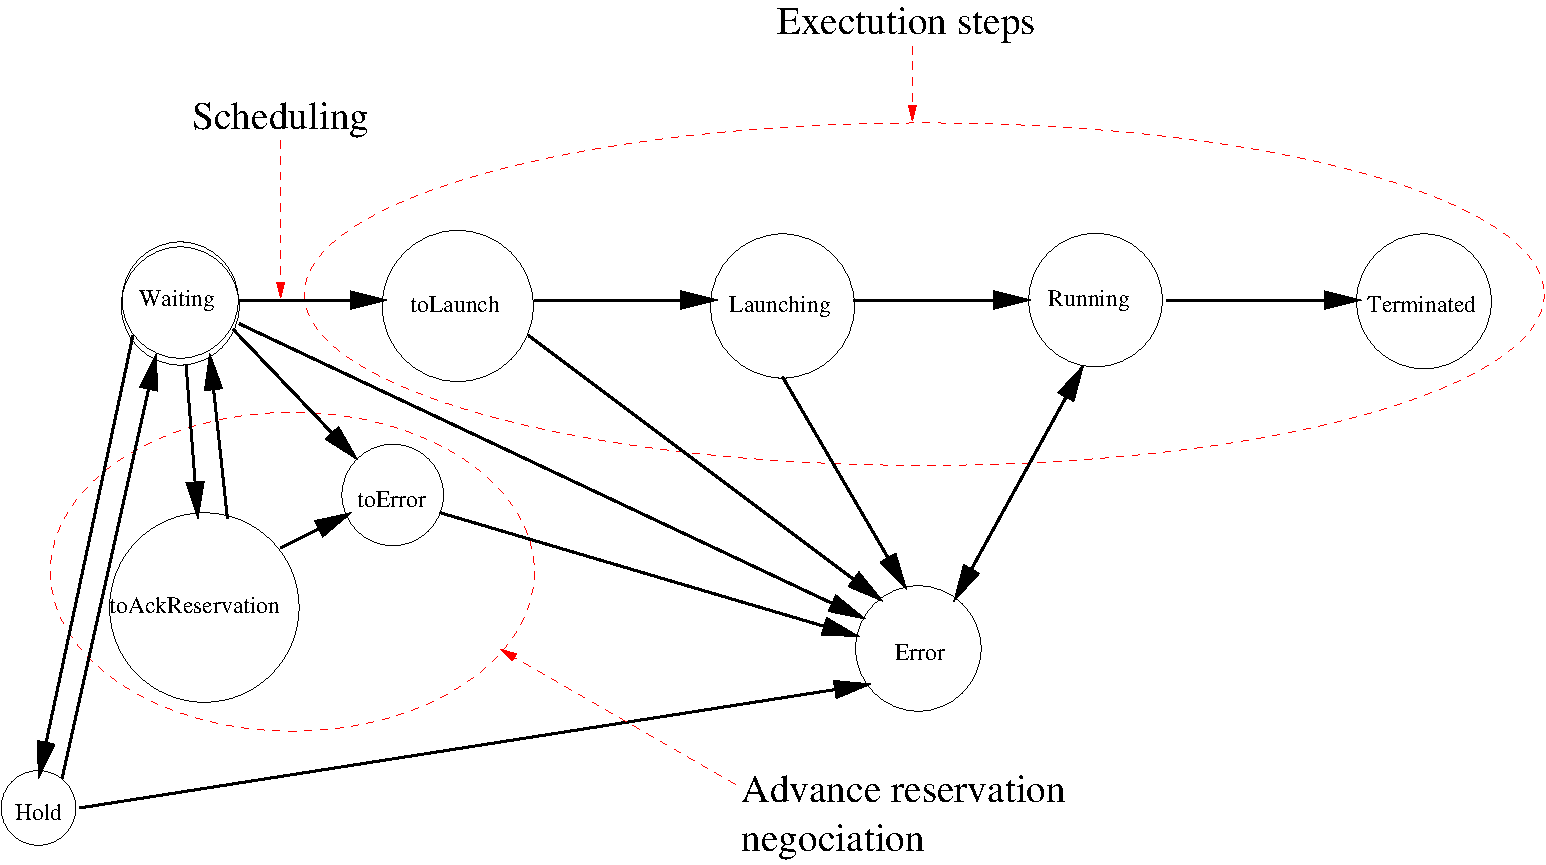
\includegraphics[width=\textwidth]{JobStates.pdf}
}

\begin{frame}
	\frametitle{Submission examples: OAR}
	
Interactive task: \footnote{{\bf Note:} Each submission command returns an id number.}

		\begin{itemize}
			\item	{\bf oarsub -l nodes=4 -i}
		\end{itemize}

	{\em Batch} submission (with {\em walltime} and choice of the queue):
		\begin{itemize}
			\item	{\bf oarsub -q default -l walltime=2:00,nodes=10 /home/toto/script}
		\end{itemize}

	Advance reservation:
		\begin{itemize}
			\item	{\bf oarsub -r "2008-04-27 11:00" -l nodes=12}
		\end{itemize}

	Connection to a reservation (using task's id):
		\begin{itemize}
			\item	{\bf oarsub -C 154}
		\end{itemize}


\end{frame}

\section{Scheduling}

% FIFO, BACKFILLING, FAIRSHARING, Advance reservartion, PRIORITE, BEST-EFFORT récursivité

\begin{frame}
	\frametitle{Scheduling}
	
	Scheduling is the step \footnote{{\bf Note:} scheduling is computed again at each major change in the state of a task.}
at which the system selects the {\bf ressources to give} to tasks {\bf and starting dates}.
\\[0.4cm]
	Scheduling is made following a {\bf policy} that is defined by a {\bf scheduling algorithm}.
\\[0.4cm]
	{\bf Furthermore} numerous {\bf parameters} are used to guide and scope the allocations and priorities.
 

\end{frame}

\frame{
	\frametitle{Scheduling organization into OAR}
	Tasks are put into queues
	\begin{itemize}
		\item each queue as a priority level
		\item each queue obey to a scheduling policy
	\end{itemize}
%equivalent to scheduling jobs with priorities but easier to administrate
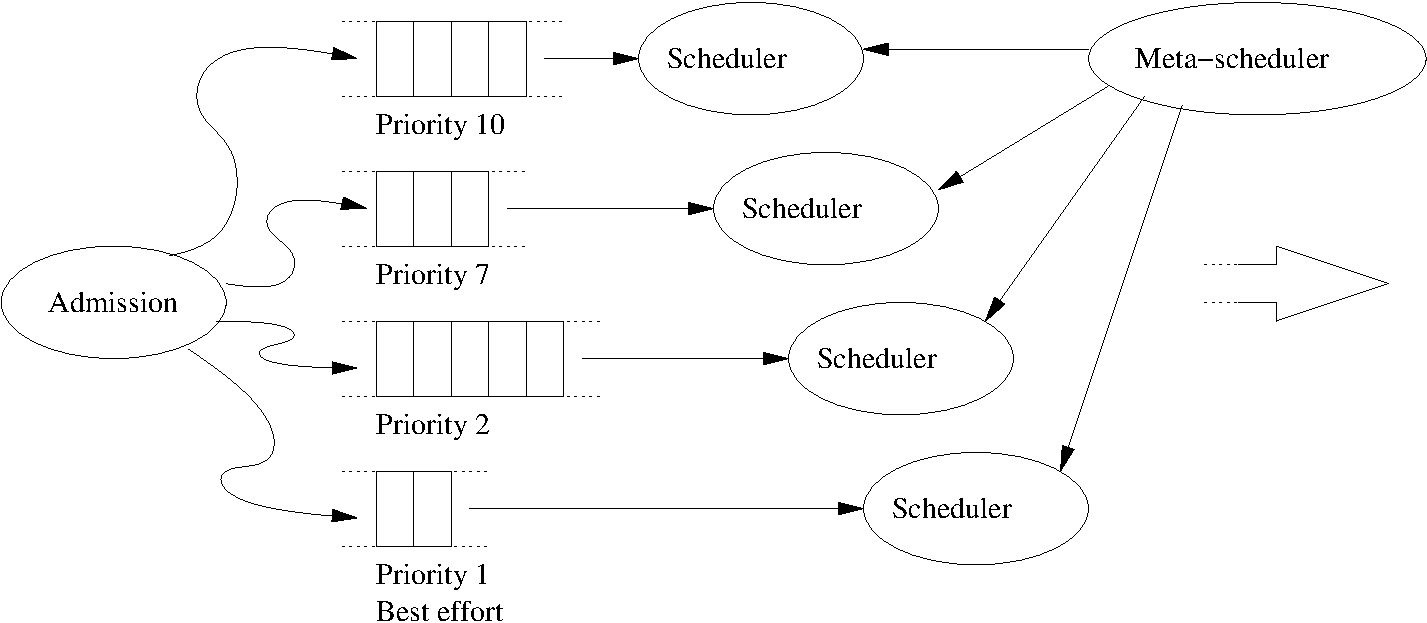
\includegraphics[width=\textwidth]{schedule_eng.pdf}
}

\frame{
	\frametitle{Resource matching}

  \begin{block}{A preliminary step to scheduling}
    \begin{itemize}
      \item Resources {\bf filtering}
      \item Resources {\bf sorting} 
      \item Allows the user to have special needs
      \item memory, architecture, special hosts, OS, workload...    
    \end{itemize}
  \end{block}

%  Condor / ClassAds : Syntaxe, Attributs, Opérateurs, Classement (Ranking)
}




\begin{frame}
	\frametitle{Scheduling policies}
		\begin{itemize}
		\item FIFO (First-In First-Out)
		\item First-Fit (Backfilling)
		\item FairSharing
		\item Timesharing
		\item Advance reservation
		\item Recursivity
	\end{itemize}

\end{frame}

\begin{frame}
	\frametitle{FIFO: Fisrt-In First-Out}
	\begin{center}
		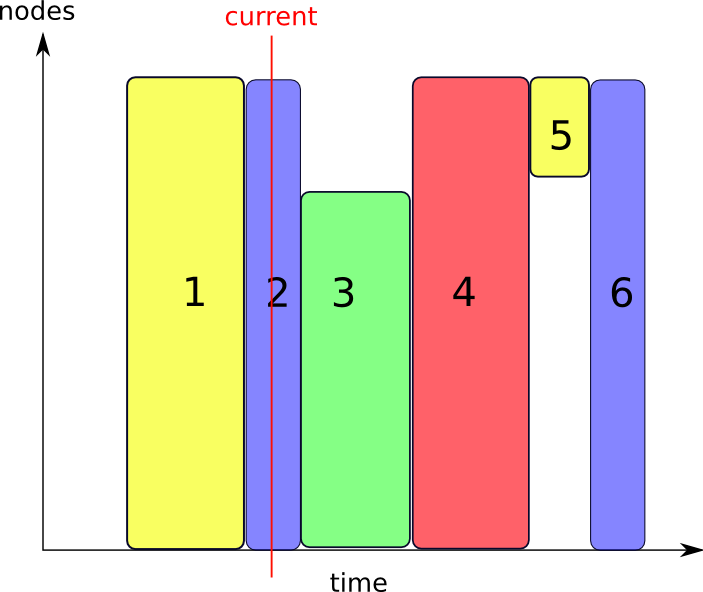
\includegraphics[width=7cm]{fifo.png}
	\end{center}

\end{frame}

\begin{frame}
	\frametitle{ First-Fit (Backfilling)}
        Holes are filled if the previous tasks order is not changed.
	\begin{center}
			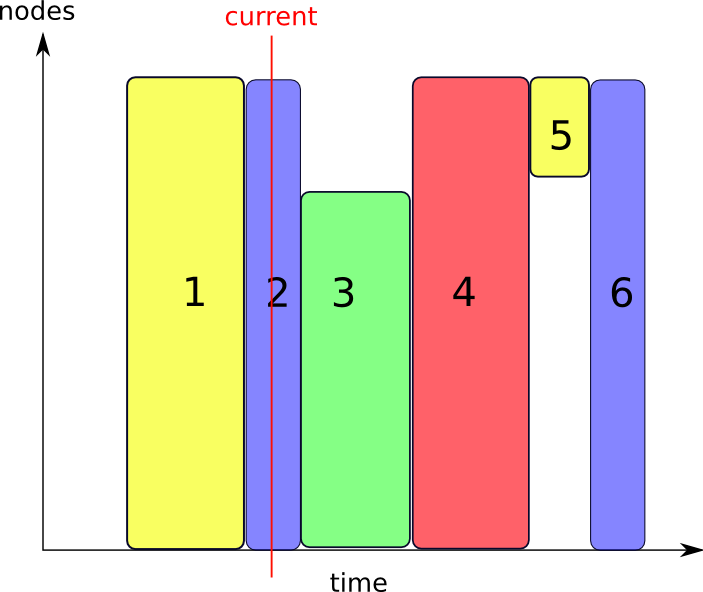
\includegraphics[width=6cm]{fifo.png}
		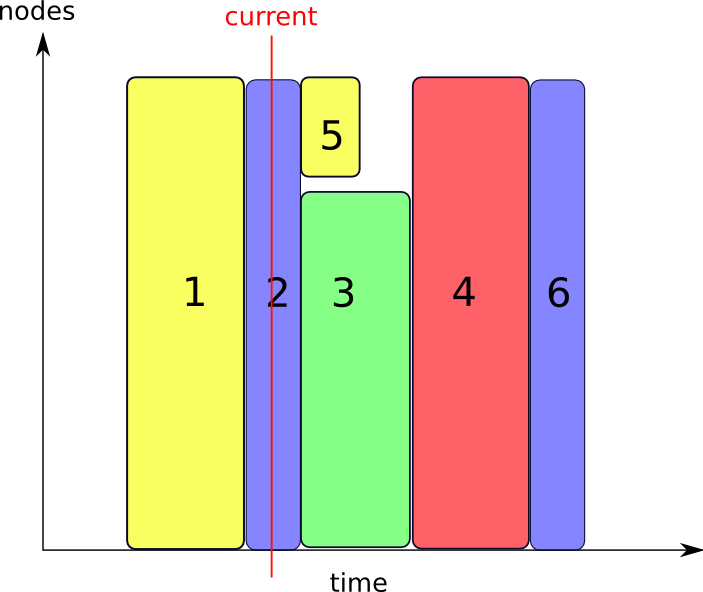
\includegraphics[width=6cm]{cbf.png}
	\end{center}

\end{frame}

\begin{frame}
	\frametitle{FairSharing}
        The order of tasks is computed depending on what has already been consumed (low time-consuming users are prioritized)
	A time-window and weighting parameters are defined.
	\begin{center}
		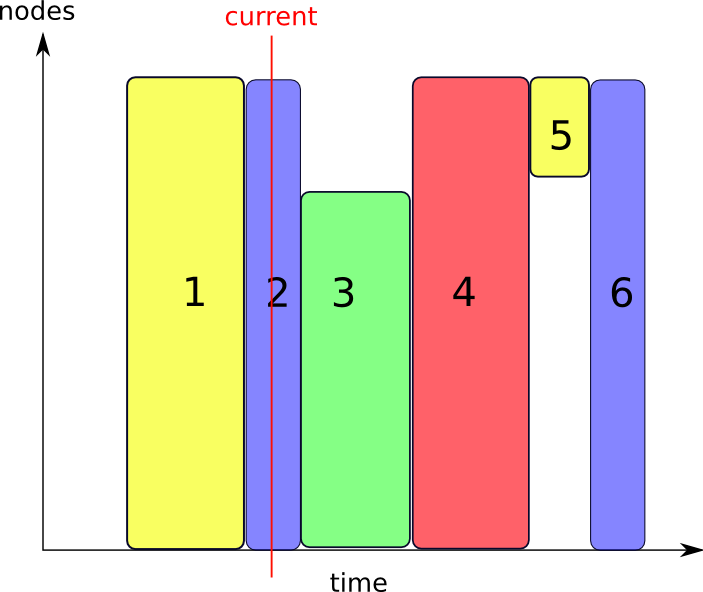
\includegraphics[width=6cm]{fifo.png}
		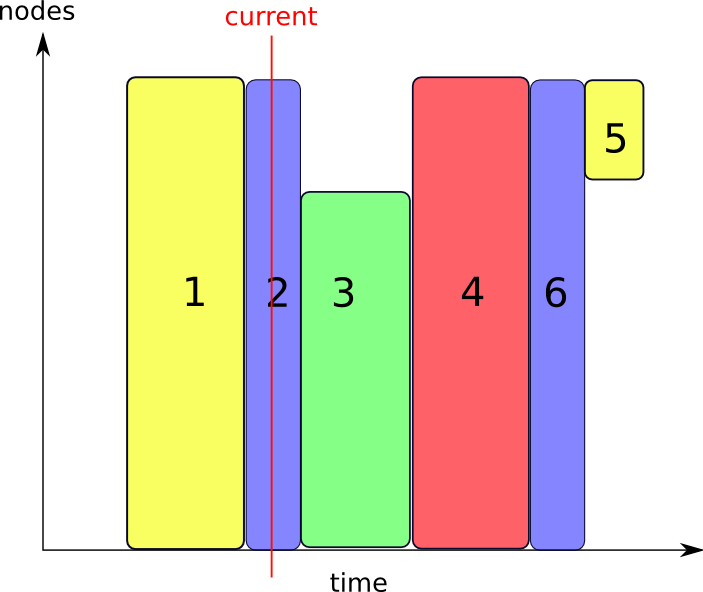
\includegraphics[width=6cm]{fairsharing.png}
	\end{center}
\end{frame}

\begin{frame}
	\frametitle{{\em Advance Reservation}}

		\begin{itemize}
		\item {\bf Very useful} for demos, planification, multi-site tasks or grid tasks...
		\item {\bf But:}
			\begin{itemize}
				\item Restrictive for the scheduling
				\item Resources are rarely used along the whole duration of the reservation (waste!)
			\end{itemize}
		\end{itemize}

	\begin{center}
		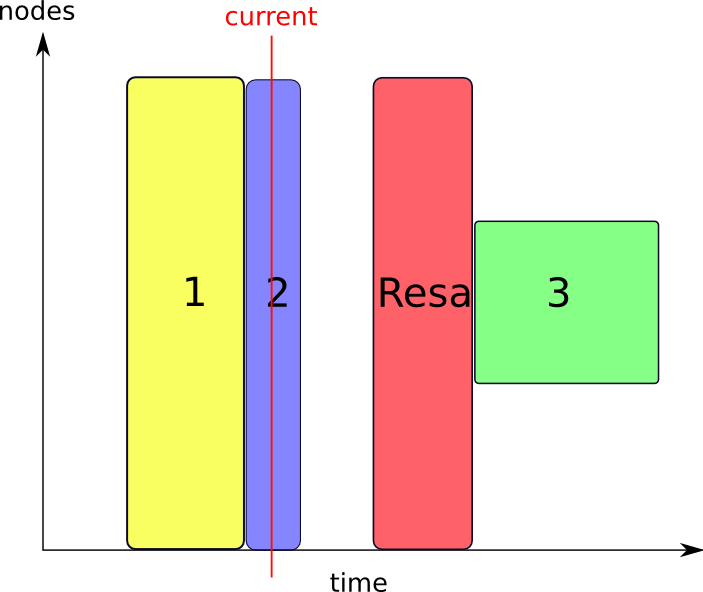
\includegraphics[width=6cm]{resa.png}
	\end{center}
	{\bf oarsub -r "2008-04-27 11:00" -l nodes=12}

\end{frame}

\begin{frame}
  \frametitle{TimeSharing} 
  \begin{center}
			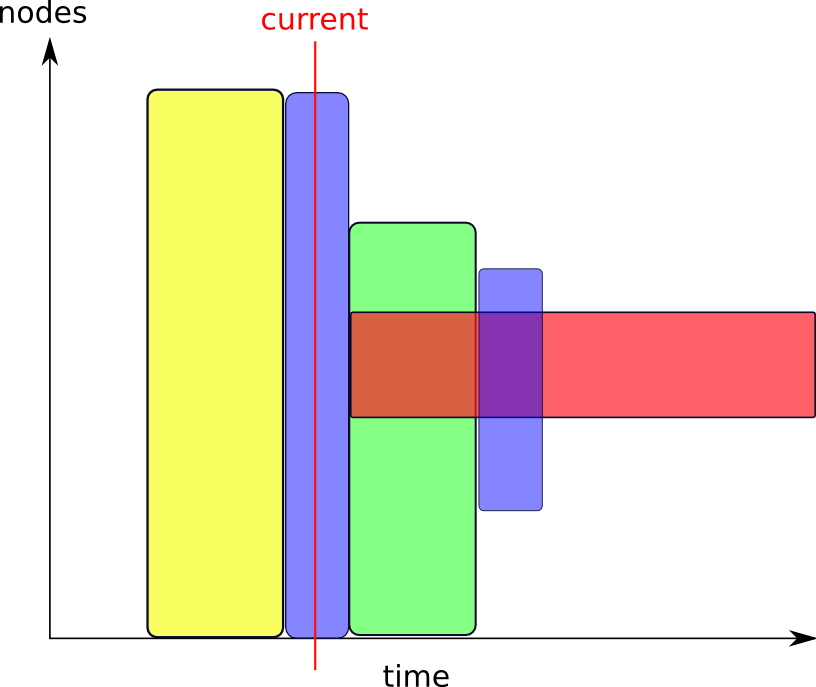
\includegraphics[width=7cm]{timesharing.png}
	\end{center}
\end{frame}

\begin{frame}
  \frametitle{Recursivity}
  Scheduling inside an allocation or a reservation. Interesting for schools, demos, flexible resources sharing inside groups of users or projects.  {\bf Container} type of task. 
  \begin{center}
			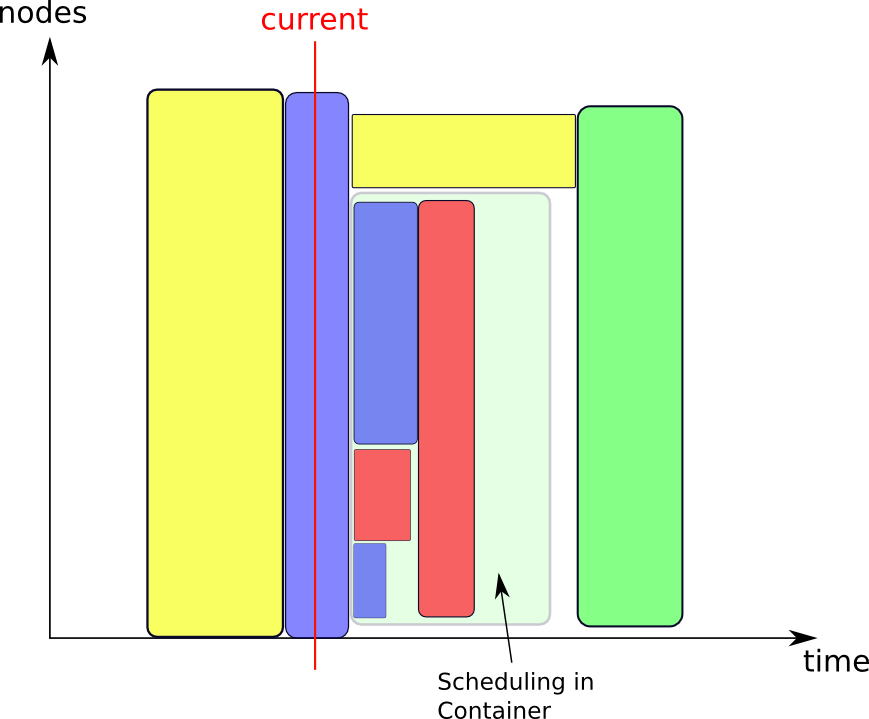
\includegraphics[width=7cm]{recursivity.png}
	\end{center}

\end{frame}

\section{Topological constraints}

\frame{
\frametitle{Topological constraints} \hypertarget{topo}{}
  \begin{block}{Hardware evolution}
    \begin{itemize}
      \item switch/node/cpu/core: \alert{Hierarchical architecture}
      \item NUMA host/ BlueGene host: \alert{2D grid, 3D or hybrid} \hyperlink{topo-appendix}{ \beamergotobutton{...}}
    \end{itemize}
  \end{block}
  \begin{center}
  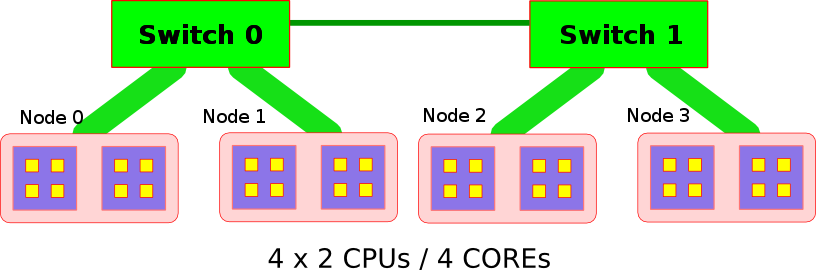
\includegraphics[width=9cm]{img/cluster_hierar.png}
  \end{center}
}

\frame{
\frametitle{Contraintes Topologiques: grille/tore 2D} \hypertarget{topo-appendix}{}
\begin{center}
  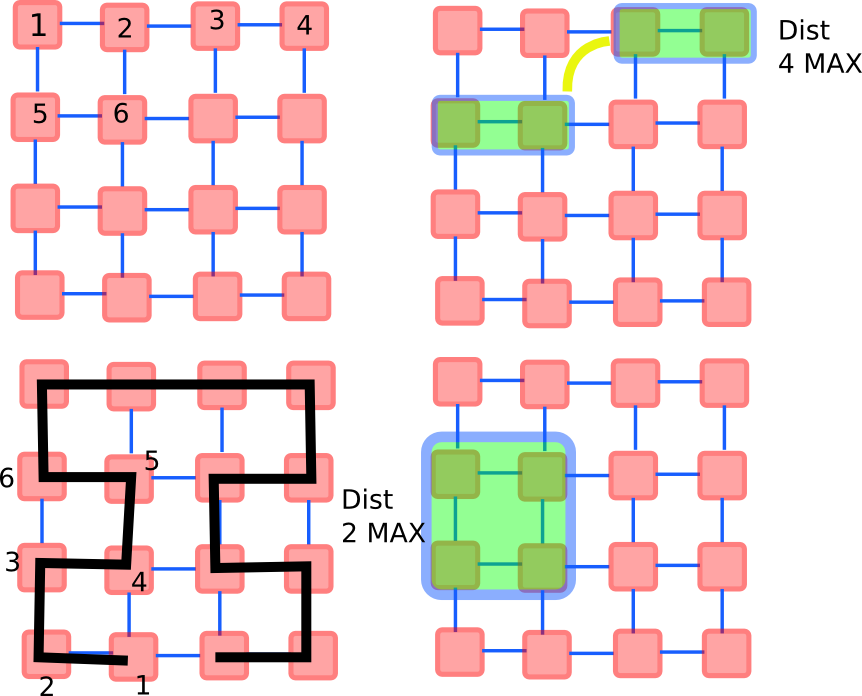
\includegraphics[width=9cm]{img/grille_2D_renum.png}
\end{center}
}

\frame{
\frametitle{Contraintes Topologiques: grille/tore 3D}
\begin{itemize}
  \item Courbe de Hilbert (Slurm / topology)
  \item Wikipedia / $Hilbert\_curve$ 
\end{itemize}
\begin{center}
  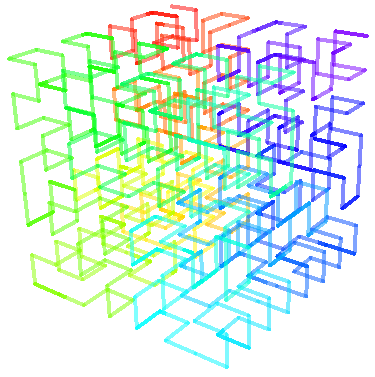
\includegraphics[width=5cm]{img/Hilbert3d-step3.png}
\end{center}
\hyperlink{topo}{\beamerreturnbutton{Back.}}
}


\frame{
\frametitle{Hierarchical topological constraints}
Problem with parallel applications that are network-bandwidth sensitive.
\begin{center}
  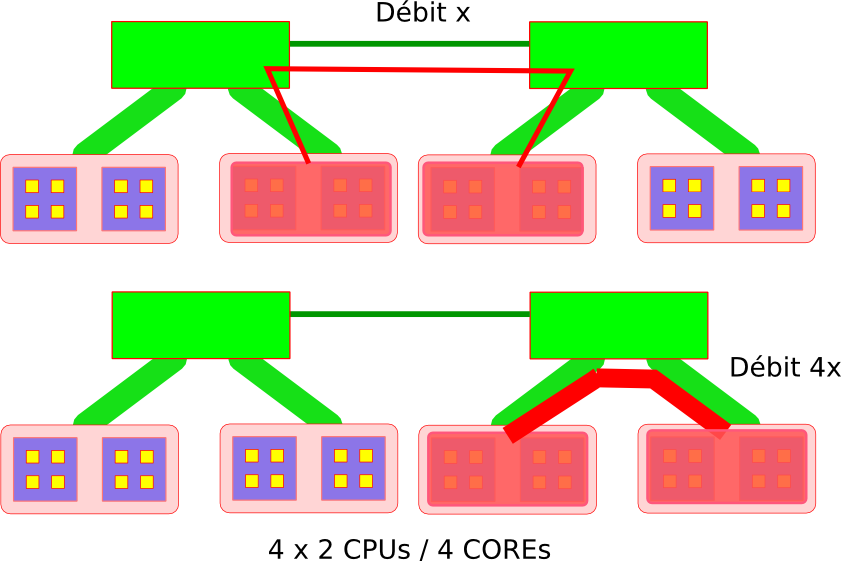
\includegraphics[width=9cm]{img/cluster_hierar_app.png}
  \end{center}
}

\frame{
\frametitle{Hierarchical topological constraints}

\begin{itemize}
 \item Hierarchy in the requests:
  \\
  {\bf oarsub -l switch=1/nodes=2/cpu=2/core=2 ./my-app}
   \\        = 1x2x2x2 = 8 cores
 \item Linux cpusets management (be aware of the cpu affinity inside a cpuset)
\end{itemize}
}


\frame{
  \frametitle{Parallel application and processor affinity}
 
  {\bf Note:} CPUSET: core/cpu/mem sub-group inside a node.

\begin{block}{}

	  \begin{enumerate}
      \item L'attribution CPUSET/core pour application parallèle peut ne pas suffire
      \item Problème de l'ordonnanceur de l'OS (ici souvent Linux), le processus change de coeur à l'intérieur des CPUSET 
 		  \item Il faut utilisé les capacités de verrouillage sur coeur ({\em Processor Affinity})
	  \end{enumerate}

\end{block}
 
}

%%% TODO
%%% Energie
%%% Tolérance aux pannes
%%% API
%%% GUI

\section{Energy}

\begin{frame}
  \frametitle{Energy saving} \hypertarget{energy}{}
  \begin{itemize}
    \item {\bf We can shutdown nodes when not used (on-demand wake up)}
    \item Timetable priorities
		\item Work done during {\em Google Summer Of Code 2008} (Gsoc'08)
    \begin{itemize}
       \item Parametrical job type:  {\bf powersaving} + options (cpufreq, disk shutdown, video ..., special policy)
       \item Ex Job BestEffort $\rightarrow$ lowest CPU frequency.
    \end{itemize}
  \end{itemize}
  \begin{center}
    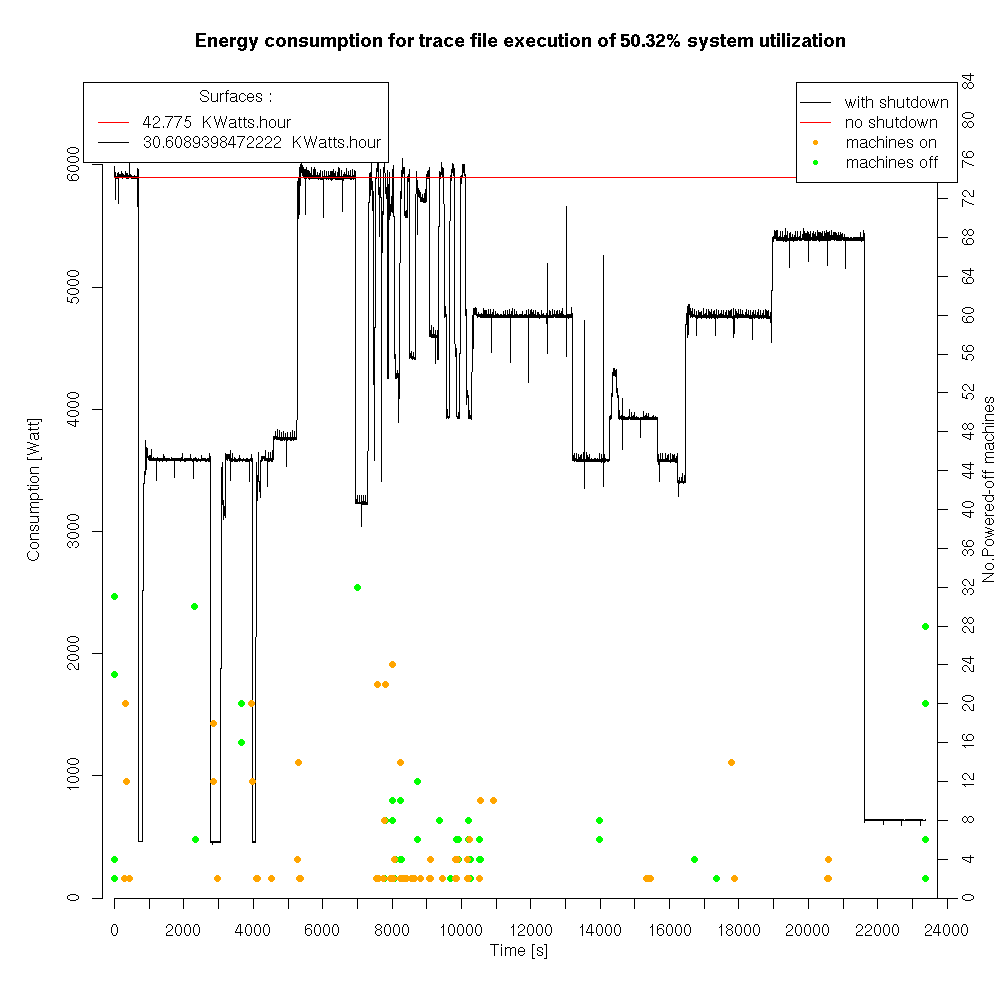
\includegraphics[width=3cm]{img/energy50.png}
    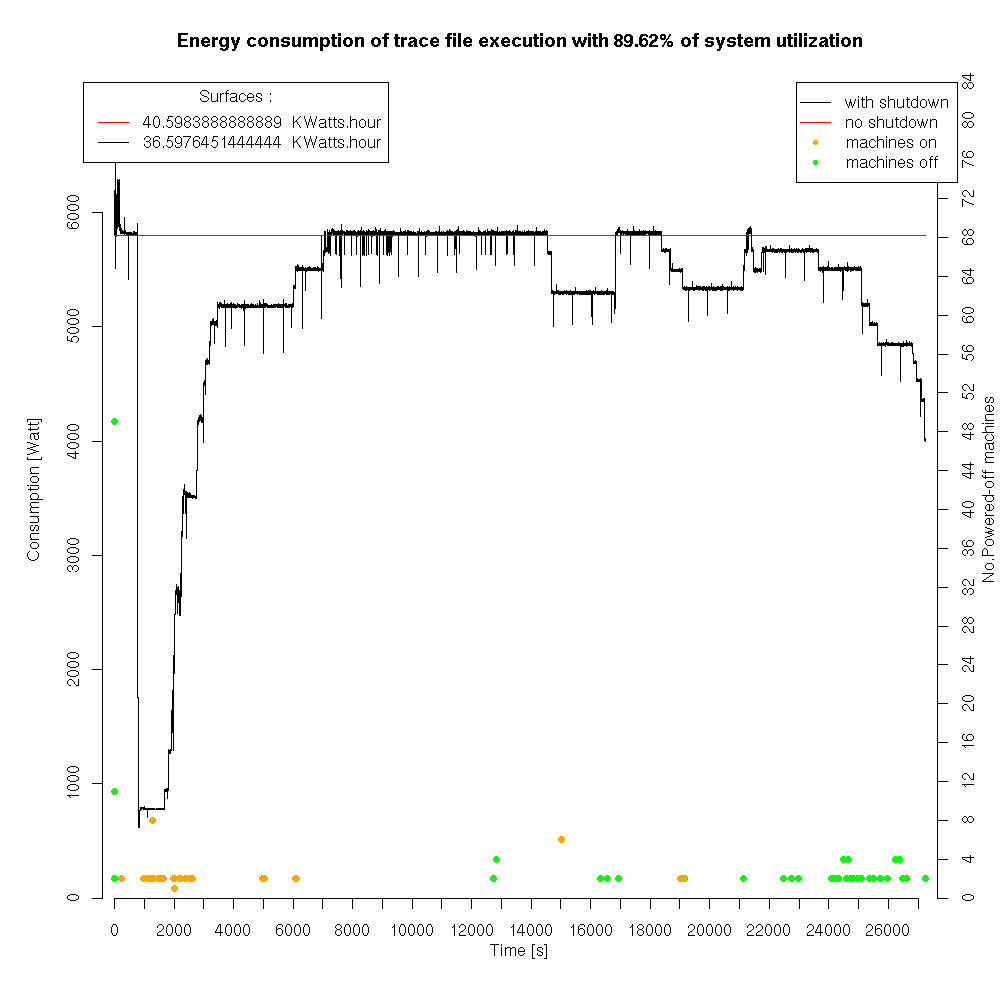
\includegraphics[width=3cm]{img/energy90.png}
    \\\hyperlink{energy-appendix}{\beamergotobutton{...}}
  \end{center}
\end{frame}


\section{Interfaces}

\frame{
  \frametitle{OAR: Monika}
  \begin{center}
  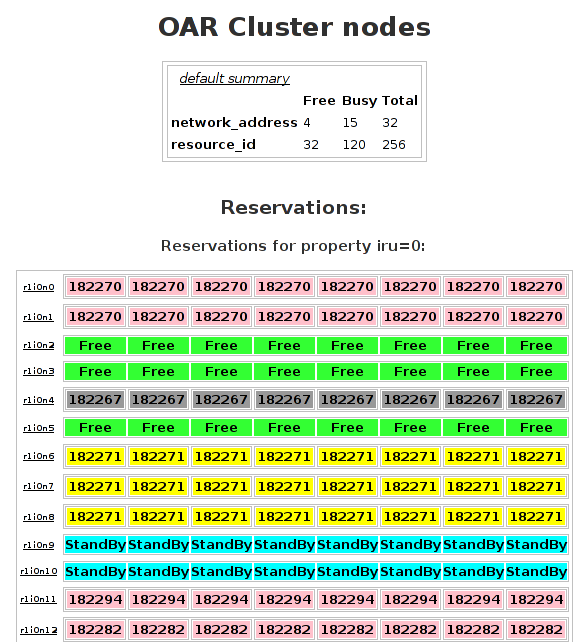
\includegraphics[width=7cm]{img/monika.png}
  \end{center}
}


\frame{
  \frametitle{OAR: Gantt diagramm}
  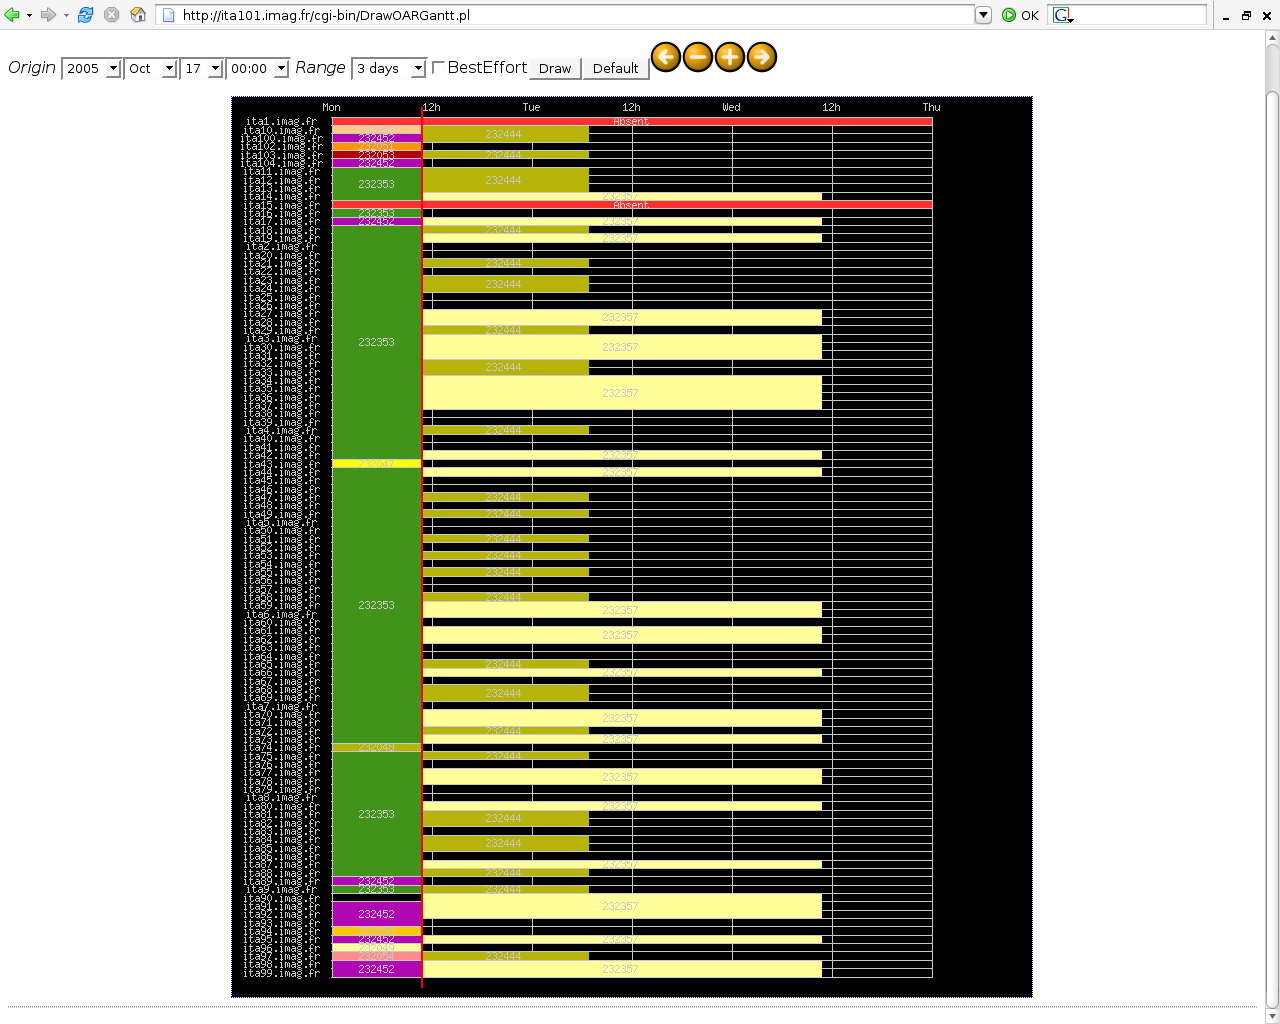
\includegraphics[width=\textwidth]{gantt_ita.png}
}


\begin{frame}
  \frametitle{REST API}

  \begin{block}{}
    \begin{itemize}
      \item REST = HTTP PUT/GET/POST/DELETE on resources 
      \item {\bf Very easy and powerful interface !}
      \item Not heavy as Web Services à la Soap.  
    \end{itemize}
  \end{block}

  \begin{block}{}
    \begin{itemize}
      \item {\bf  \url{http://mydomain.org/oarapi/resources.json} }
      \item  Gives the list of every resources in the json format 
    \end{itemize}
  \end{block}
      wget -O - http://mydomain.org/oarapi/resources.yaml?structure=simple

\end{frame}

\frame{
  \frametitle{REST API usage example}
  \begin{center}
    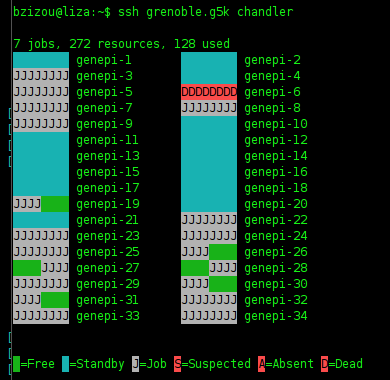
\includegraphics[width=6cm]{img/chandler2.png}
  \end{center}
  {\em Chandler}: only 80 lines of code, prints the status of nodes and cores with colors in a command line shell
}


\section{Future works and conclusion}

\frame{
  \frametitle{The team }
  \begin{block}{The OAR team}
  \begin{itemize}
    \item {\bf 1 senior engineer (\%50) + 2 contract engineers + 1 phd student}
    \item {\bf 1 researcher (direction, coding) + 3 researchers (consultants / occasional coding)}
    \item Contributors (including the former principal developper)
    \item 5 interns Gsoc (Google Summer of Code 08 et 09) 
    \item About 10 people who contributed
  \end{itemize}
 \end{block}
}

\frame{
  \frametitle{References/support}

  \begin{block}{References}
  \begin{itemize}
    \item Between 7000 and 15000 cores, about 30 clusters
    \item Mesocentre CIMENT, Grid'5000, BRGM, Footways, Usharesoft, Université/Labo (France, Chine, Brésil,Luxembourg, US, Slovakie...)
  \end{itemize}
 \end{block}

  \begin{block}{Support}
  \begin{itemize}
    \item OAR Licence GPL
    \item Mailing List, Bugzilla
    \item Installation support (us or a partner ex: BULL/Serviware)
    \item Pro support (to be discussed)
  \end{itemize}
 \end{block}
}

\frame{
  \frametitle{Future works}
  \begin{block}{}
  \begin{itemize}
    \item {\bf gLite interfacing} (server blahp ?)
    \item {\bf Scheduler (new version)}
    \item Integrated web interface
    \item Virtual cluster: Boinc coupling / Computemode revival
    \item Test environment / re-play
    \item Currently 1000 to 10000 (resources: nodes, cpus, cores...)
    \item 100K resources, numa massively multi-core  ?
    \item inefficienties detection ?
    \item Partenariats BULL, CEA
  \end{itemize}
 \end{block}



}

\frame{
  \frametitle{Conclusion}

 \begin{block}{}
  \begin{itemize}
    \item {\bf Versatile and customizable}
    \item Features level like other products
    \item Very stable
    \item Current stable version:  {\bf {\em 2.4.1 (Thriller)}} (.tgz, .deb, .rpm)
    \item Next version in a few weeks, with a new energy saving module:  {\bf {\em 2.4.2}} (.tgz, .deb, .rpm)
    \item This is a continuously evolving domain 
  \end{itemize}
 \end{block}
 \begin{center}
    \hspace{-1.5cm}
    \includegraphics[height=9ex]{img/oar_logo.png}
   \end{center} 


}

\frame{
  \begin{center}
		{\huge Des questions ?}
	\end{center}

  \begin{center}
    \hspace{-1.5cm}
    \includegraphics[height=4cm]{img/oar_logo.png}
   \end{center} 

  \begin{center}
    \vspace{-0.5cm}
    {\bf http://oar.imag.fr/}
  \end{center}
}


\begin{frame}
\frametitle{Liens}
\begin{thebibliography}{Resource Management System}

	\bibitem{Condor}
	Condor 
	\newblock {\em http://www.cs.wisc.edu/condor/}

  \bibitem{SGE}
	Sun Grid Engine (SGE) 
	\newblock {\em http://gridengine.sunsource.net}

	\bibitem{TORQUE}
	TORQUE/MAUI
	\newblock {\em http://www.clusterresources.com/}

  \bibitem{SLURM}
	SLURM
	\newblock {\em www.llnl.gov/linux/slurm/}

	\bibitem{LSF}
	LSF
	\newblock {\em http://www.platform.com}

	\bibitem{OAR}
	OAR 
	\newblock {\em http://oar.imag.fr}



\end{thebibliography}
\end{frame}


\section{Annexes}

\frame{
\frametitle{OAR: Historique}
%%% TODO rajoute image icluster
\begin{itemize}
  \item Début 2003: Une machine dans le Top500 (225 noeuds), OpenPBS(Torque) est instable et difficile à faire évoluer 
  \item PBSpro se comporte mieux (passage à l'échelle imparfait)
\end{itemize}

	\begin{center}
  	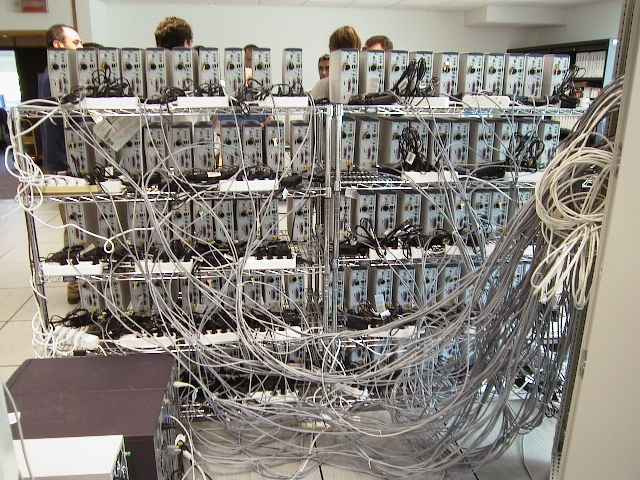
\includegraphics[width=6cm]{img/icluster1.jpg}
  \end{center}
}

\frame{
\frametitle{Contraintes Topologiques: grille/tore 2D} \hypertarget{topo-appendix}{}
\begin{center}
  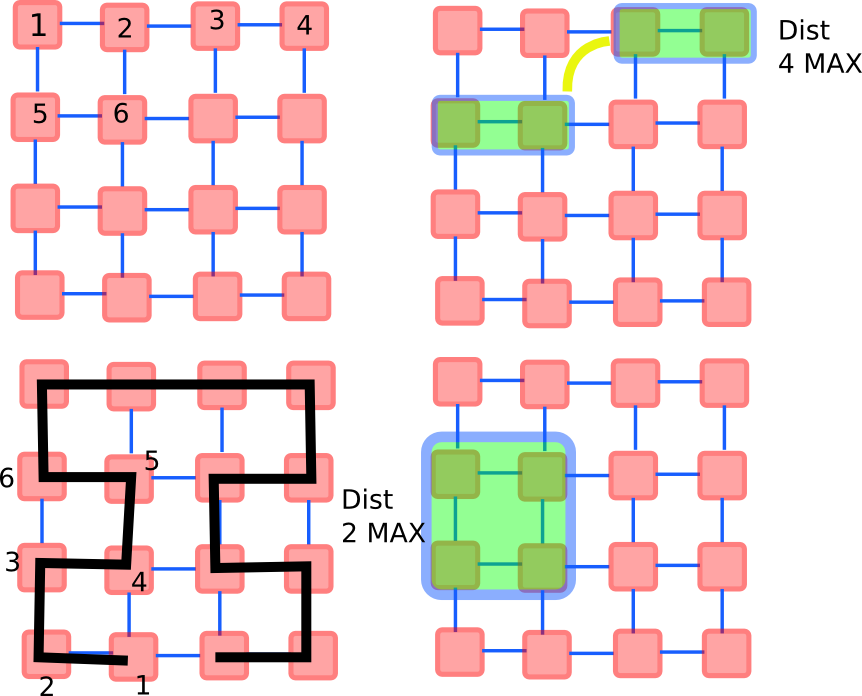
\includegraphics[width=9cm]{img/grille_2D_renum.png}
\end{center}
}

\frame{
\frametitle{Contraintes Topologiques: grille/tore 3D}
\begin{itemize}
  \item Courbe de Hilbert (Slurm / topology)
  \item Wikipedia / $Hilbert\_curve$ 
\end{itemize}
\begin{center}
  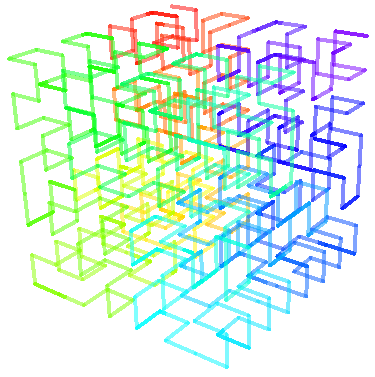
\includegraphics[width=5cm]{img/Hilbert3d-step3.png}
\end{center}
\hyperlink{topo}{\beamerreturnbutton{Back.}}
}

\frame{
\frametitle{Interfaces:}

\begin{block}{}
  \begin{itemize}
    \item Interface commande en ligne (CLI)
    \item Application exemple DRMAA (v1, v2)
    \item Grille : Globus GT2, GT4/ OGSA-BESS, JSDL, G-Lite - BLAHp, SAGA
    \item Beaucoup d'interface, souvent limitatives ?
  \end{itemize}
 \end{block}

	\begin{center}
			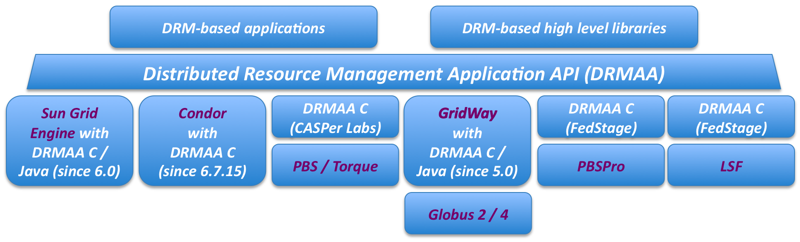
\includegraphics[width=9cm]{img/drmaastack.png}
	\end{center}

  {\bf OAR}: DRMAA (85\%), Glite ({\bf commandée}), REST

}


\frame{ \hypertarget{energy-appendix}{}
	\begin{center}
    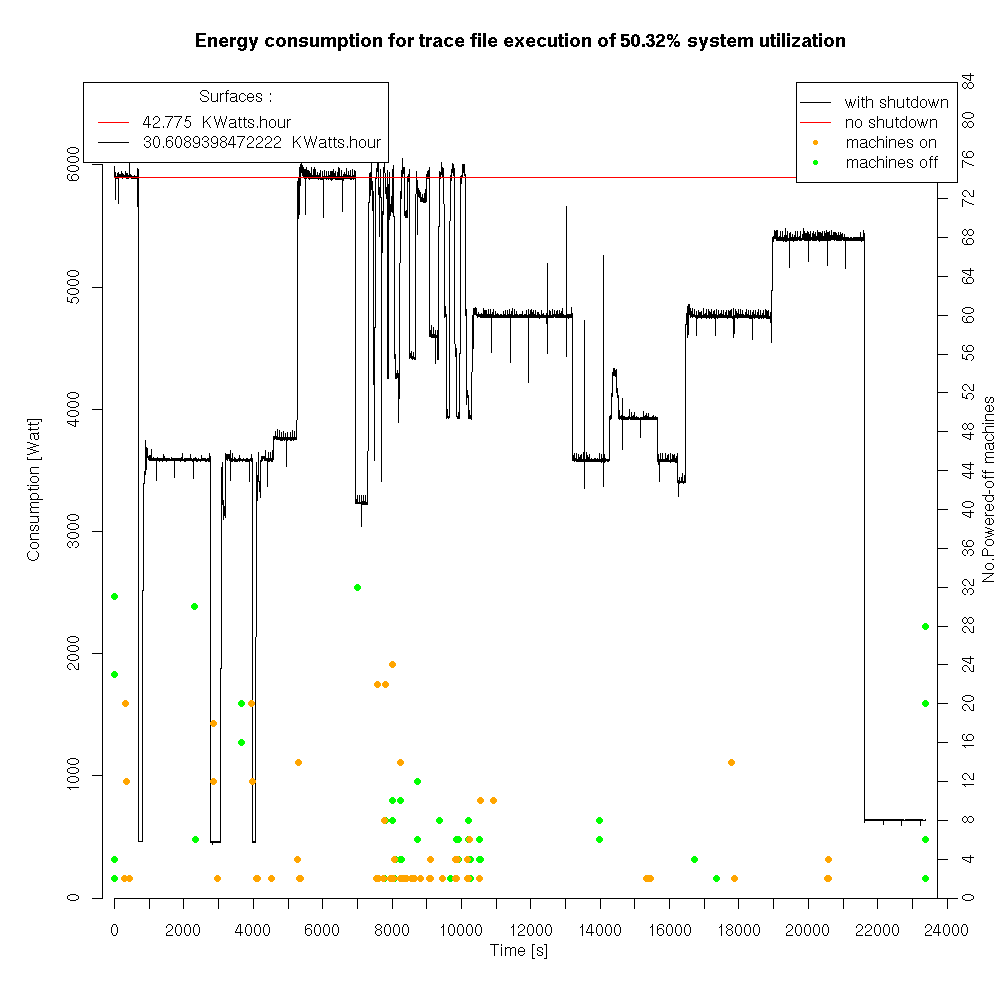
\includegraphics[width=9cm]{img/energy50.png}
  \end{center}
}

\frame{
  \begin{center}
    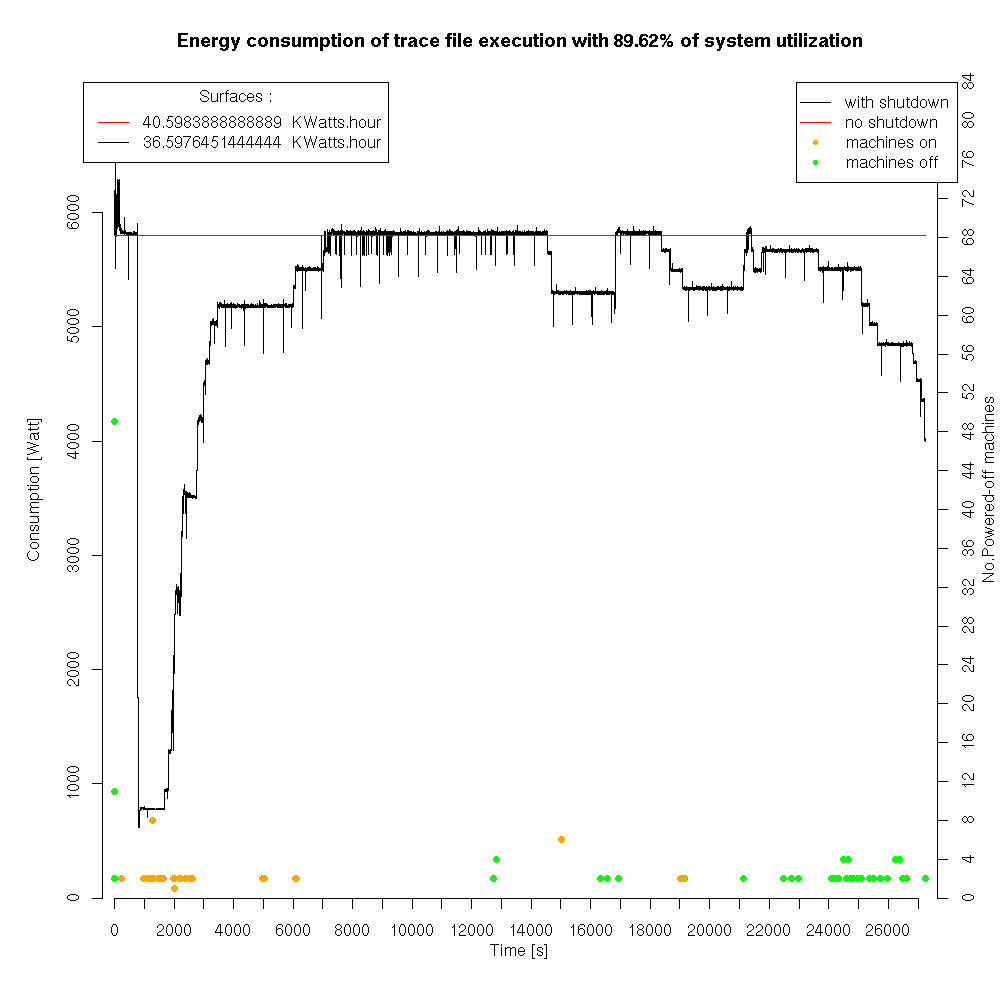
\includegraphics[width=8cm]{img/energy90.png}
  \end{center}
\hyperlink{energy}{\beamerreturnbutton{Back.}}
}

\end{document}

